\qquad A análise de complexidade do Bubble Sort, considerando as
diferentes situações de entrada (crescente, decrescente e
randômica), foi realizada manuscrita, com a devida justificativa,
contando o número de execuções de cada linha do algoritmo, no mesmo
formato adotado nos capítulos anteriores, conforme exigido pelo
enunciado do trabalho.

\begin{figure}[htbp]
    \centering
    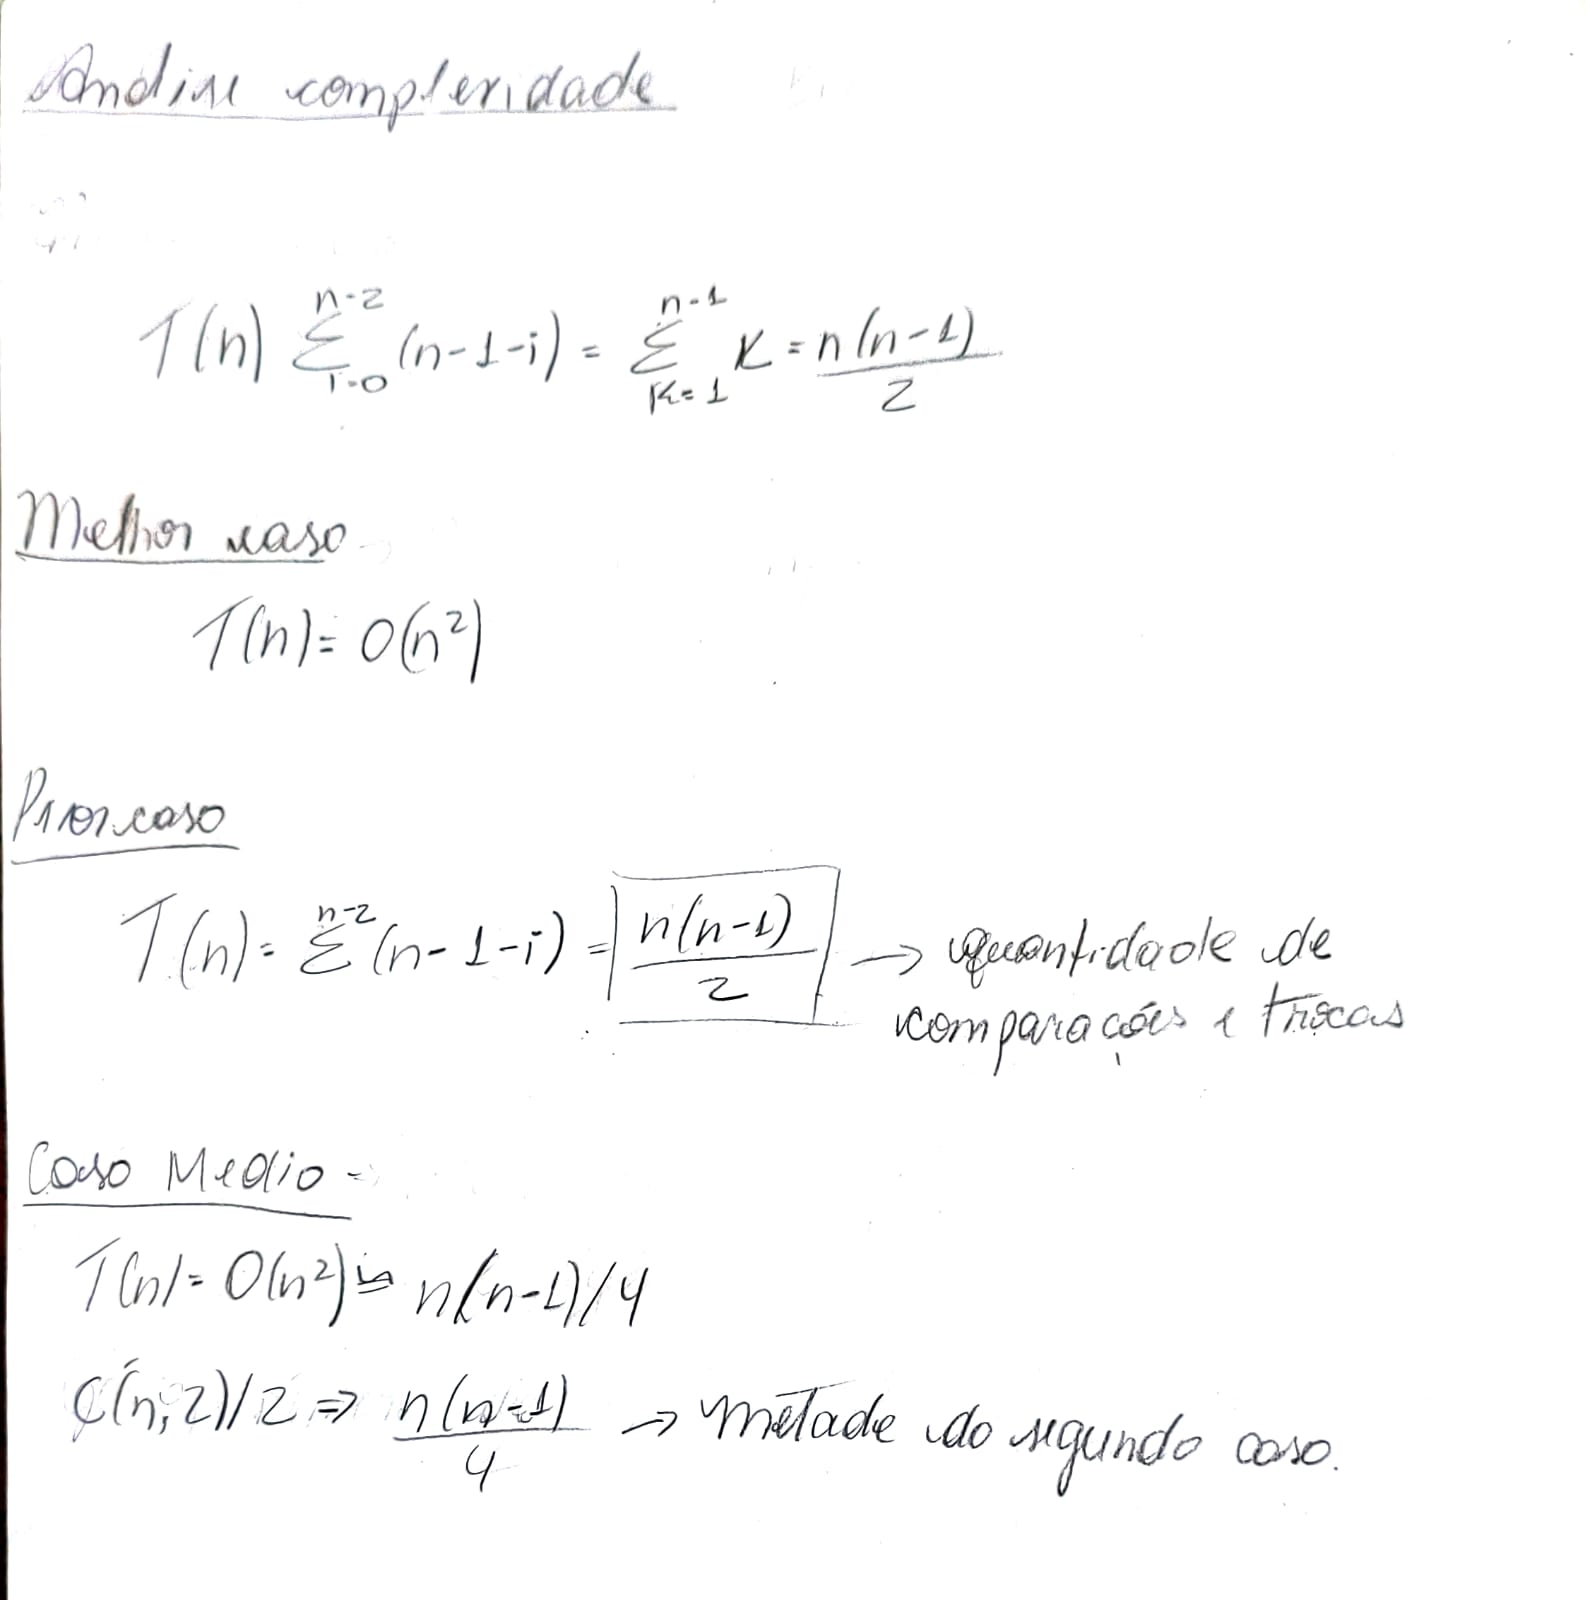
\includegraphics[width=14cm]{Imagens/Bubble Sort/analise_complexidade.jpeg}
    \caption{Análise de complexidade manuscrita do algoritmo Bubble Sort}
    \label{fig:analise_complexidade_bubble}
\end{figure}

\qquad Em resumo, a análise manuscrita chega às seguintes conclusões
para cada situação de entrada, considerando a otimização de parada
antecipada (\textit{flag} de troca) implementada:

\textbf{Melhor caso (entrada crescente):} a primeira passada não
realiza nenhuma troca, o que aciona a parada antecipada; apenas
$n-1$ comparações são feitas, logo $T(n) = O(n)$.

\textbf{Caso médio (entrada randômica):} o número de comparações
permanece $\approx \frac{n(n-1)}{2}$ (a parada antecipada raramente
ocorre antes da última passada), mas o número esperado de trocas cai
para cerca de metade do pior caso, $\frac{n(n-1)}{4}$ — o mesmo
raciocínio de inversões esperadas usado no caso médio do Insertion
Sort (Capítulo 1). Ainda assim, $T(n) = \Theta(n^2)$.

\textbf{Pior caso (entrada decrescente):} todas as $n-1$ passadas são
necessárias, cada uma com o número máximo de comparações e trocas,
totalizando $\frac{n(n-1)}{2}$ comparações e o mesmo número de trocas,
ou seja, $T(n) = \Theta(n^2)$.

\qquad Os resultados experimentais apresentados na próxima seção deste
capítulo são compatíveis com essa análise teórica: desempenho linear
no melhor caso (entrada crescente, graças à parada antecipada) e
desempenho quadrático no caso médio e no pior caso (entradas
randômica e decrescente). Vale destacar que, apesar de Insertion Sort e Bubble Sort compartilharem a mesma ordem de grandeza no pior caso, cada troca do Bubble Sort custa três atribuições, contra apenas uma atribuição por deslocamento no Insertion Sort, o que tende a torná-lo mais lento na prática. Os tempos medidos, porém, mostram que o custo de cada instrução não é o único fator: na entrada randômica o Bubble Sort foi cerca de 11,6 vezes mais lento que o Insertion Sort (938,7 s contra 80,6 s para 1.000.000 de elementos), enquanto na entrada decrescente os dois tiveram desempenho equivalente (155,6 s contra 167,0 s). Na entrada randômica, parte da diferença vem do número de comparações (cerca de $n(n-1)/2$ no Bubble Sort contra $n(n-1)/4$ no Insertion Sort); o restante provavelmente decorre da previsão de desvios do processador: na entrada decrescente a condição \texttt{vetor[j] > vetor[j+1]} é sempre verdadeira, um padrão que o processador prevê quase perfeitamente, ao passo que na entrada randômica ela é imprevisível e causa perdas de desempenho do \textit{pipeline}. Essa é uma explicação plausível, mas não foi verificada neste trabalho.
